% !TEX TS-program = pdflatex
% !TEX encoding = UTF-8 Unicode

% This is a simple template for a LaTeX document using the "article" class.
% See "book", "report", "letter" for other types of document.

\documentclass[11pt]{article} % use larger type; default would be 10pt

\usepackage[utf8]{inputenc} % set input encoding (not needed with XeLaTeX)

%%% Examples of Article customizations
% These packages are optional, depending whether you want the features they provide.
% See the LaTeX Companion or other references for full information.

%%% PAGE DIMENSIONS
\usepackage{geometry} % to change the page dimensions
\geometry{a4paper} % or letterpaper (US) or a5paper or....
% \geometry{margin=2in} % for example, change the margins to 2 inches all round
% \geometry{landscape} % set up the page for landscape
%   read geometry.pdf for detailed page layout information

\usepackage{graphicx} % support the \includegraphics command and options
% \usepackage[parfill]{parskip} % Activate to begin paragraphs with an empty line rather than an indent
\usepackage{amssymb}
%%% PACKAGES
\usepackage{booktabs} % for much better looking tables
\usepackage{array} % for better arrays (eg matrices) in maths
\usepackage{paralist} % very flexible & customisable lists (eg. enumerate/itemize, etc.)
\usepackage{verbatim} % adds environment for commenting out blocks of text & for better verbatim
\usepackage{subfig} % make it possible to include more than one captioned figure/table in a single float
% These packages are all incorporated in the memoir class to one degree or another...
\usepackage{pgfplots}
%%% HEADERS & FOOTERS
\usepackage{fancyhdr} % This should be set AFTER setting up the page geometry
\pagestyle{fancy} % options: empty , plain , fancy
\renewcommand{\headrulewidth}{0pt} % customise the layout...
\lhead{}\chead{}\rhead{}
\lfoot{}\cfoot{\thepage}\rfoot{}

%%% SECTION TITLE APPEARANCE
\usepackage{sectsty}
\allsectionsfont{\sffamily\mdseries\upshape} % (See the fntguide.pdf for font help)
% (This matches ConTeXt defaults)
\usepackage[thinc]{esdiff}
%%% ToC (table of contents) APPEARANCE
\usepackage[nottoc,notlof,notlot]{tocbibind} % Put the bibliography in the ToC
\usepackage[titles,subfigure]{tocloft} % Alter the style of the Table of Contents
\renewcommand{\cftsecfont}{\rmfamily\mdseries\upshape}
\renewcommand{\cftsecpagefont}{\rmfamily\mdseries\upshape} % No bold!

%%% END Article customizations

%%% The "real" document content comes below...

\title{HW1}
\author{Wei Ye\footnote{I worked on my assignment sololy.Email: wye22@fordham.edu}  	\\
												ECON 5700}
\date{Due on August 13, 2020.}


\begin{document}
	\maketitle
	\section{Question 1}
	\textbf{Solution:}
	
	Since $|\sin(\frac{1}{x})|\leq1 \rightarrow |x^2\cdot\sin(\frac{1}{x})|\leq x^2$, in analytical language, it's bounded. 
	
	Because $\lim_{x\rightarrow0}-x^2 \leq x^2\cdot \sin(\frac{1}{x})\leq \lim_{x\rightarrow0}x^2$ , the $LHS =0$ and $RHS=0$ as well. Then by \textbf{Squeeze Theorem:} we can prove $\lim_{x\rightarrow0}x^2\sin(\frac{1}{x})=0$ $\blacksquare$

\section{Question 2}
\textbf{Solution:}

	$\lim\limits_{x\to\infty}\left(\sqrt{x^2+1}-x\right)=\lim\limits_{x\to\infty}\frac{\sqrt{x^2+1}-x}{1}\cdot\frac{\sqrt{x^2+1}+x}{\sqrt{x^2+1}+x}=\frac{x^2+1-x^2}{\sqrt{x^2+1}+x}=\lim\limits_{x\to\infty}\frac{1}{\sqrt{x^2+1}+x}=0$ $\blacksquare$
	
	
\section{Question 3}
\textbf{Solution:}

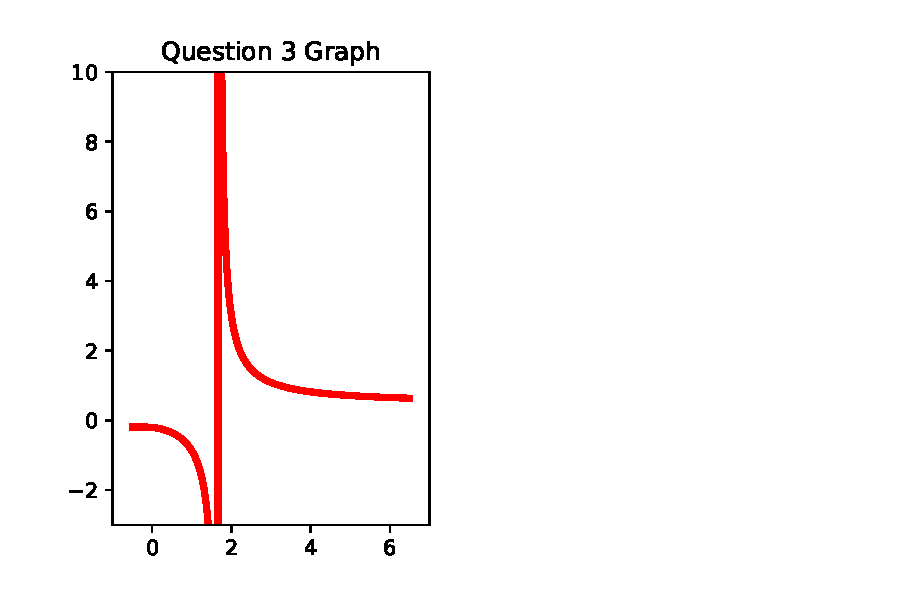
\includegraphics[width=0.4\textwidth, angle=0]{question3.pdf}



\section{Question 4}
\textbf{Solution:}

By \textbf{L' Hopital Rule:} $\lim\limits_{x\to\infty}\frac{6x-1}{10x+4}=\frac{6}{10}=\frac{3}{5}$

\section{Question 5}
\textbf{Solution:}

$\lim\limits_{x\to\infty}x^2-x=\infty$

\section{Question 6}
\textbf{Solution:}

$\lim\limits_{x\to\infty}x^3=\infty$.  $\lim\limits_{x\to-\infty}x^3=-\infty$

\section{Question 7 }
\textbf{Solution:}

By \textbf{L' Hopital's Rule:} $\lim\limits_{x\to\infty}\frac{x^2+x}{3-x}=\lim\limits_{x\to\infty}2x+1=\infty$

\section{Question 8}
\textbf{Solution:}

If $f(x)=\sqrt{x}$, then $f'(x)=\frac{1}{2\sqrt{x}}$. The domain of $f'(x)$ is $\left(0,\infty\right)$

\section{Question 9}
\textbf{Solution:}

$$f'(x)=\frac{-3}{(2+x)^2}$$


\section{Question10}
\textbf{Solution:}

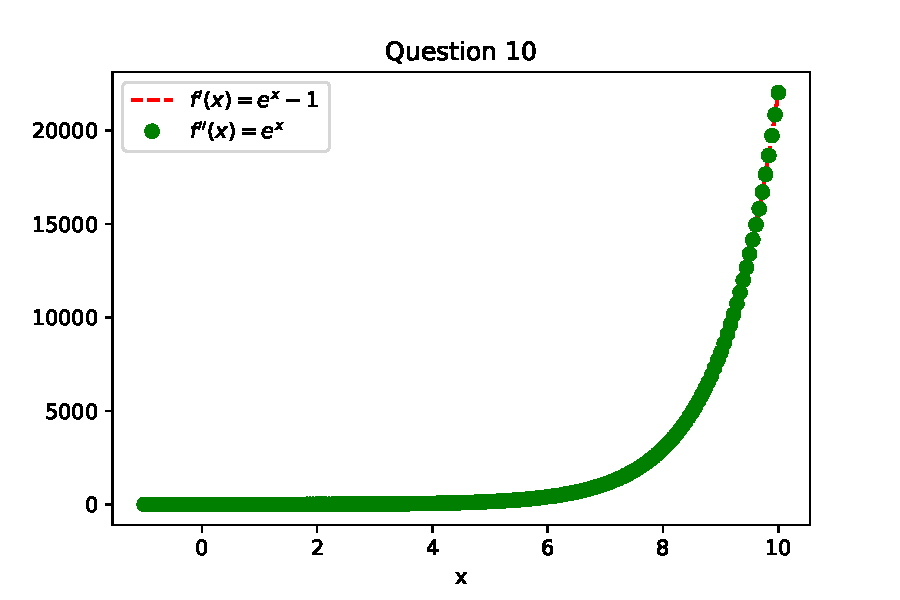
\includegraphics[width=0.4\textwidth, angle=0]{question10.pdf}

\section{Question 11}
\textbf{Solution:}

\begin{enumerate}
	\item $$f'(x)=(1+x)e^x$$
	\item $$f^{(n)}(x)=(n+x)e^x$$
\end{enumerate}

\section{Question 12}
\textbf{Solution:}

$y'=\frac{e^x(1-x)^2}{(1+x^2)^2}$, if $x=1$, then $y'=0$, and the tangent line is $y=\frac{1}{2}e$

\section{Question 13}
\textbf{Solution:}

$$g'(t)=\frac{9(t-2)^8(2t+1)^9-(t-2)^99(2t+1)^82}{(2t+1)^{18}}=\frac{45(t-2)^8}{(2t+1)^{10}}$$

\section{Question 14}
\textbf{Solution:}\footnote{Reference:https://math.stackexchange.com/questions/2485251/using-implicit-differentiation-find-y-prime-if-sinx-y-y2-cosx}

Step1: Assume a general function $F(x,y)$:
$$\frac{\partial F}{\partial x}\mathrm{d}x+\frac{\partial F}{\partial y}\mathrm{d}y=0$$
Thus:

 $$\frac{\mathrm{d}y}{\mathrm{d}x}=\frac{\frac{\partial F}{\partial x}}{-\frac{\partial F}{\partial y}}$$
 
 Step2: Specify $F(\cdot)$ in our question: $F(x,y)=\sin(x+y)-y^2\cos(x)$:
 $$y' =\frac{\cos(x+y)+y^2\sin(x)}{\cos(x+y)-2y\cos(x)}$$
 
 \section{Question $15^\star$}
 \textbf{Solution:}
 
 Step1: Take logarithms on both sides:
 $$\ln y= \ln(x^{\frac{3}{4}}(x^2+1)^{\frac{1}{2}})-\ln(3x+2)^5=\ln(x^{\frac{3}{4}})+\ln((x^2+1)^{\frac{1}{2}})-\ln(3x+2)^5$$
 
 Step2: Take differentiation on both sides w.r.t x:
 $$\frac{\mathrm{d}\ln y}{\mathrm{d}x}=\frac{3}{4x}+\sqrt{x^2+1}x+\frac{15}{3x+2}$$
 In the end:
 $$\frac{\mathrm{d}y}{\mathrm{d}x}=y\cdot\left(\frac{3}{4x}+\sqrt{x^2+1}x+\frac{15}{3x+2}\right)$$
 
 \section{Question 16}
 \textbf{Solution:}
 
 $$y=x^{x^\frac{1}{2}}$$
 Step 1: Take log on both sides:
 $$\log y= x^{\frac{1}{2}}\log x$$
 Step 2:  Take differentiation on both sides:
 $$\frac{1}{y}\frac{\mathrm{d}y}{\mathrm{d} x}=\frac{1}{2} x^{-\frac{1}{2}} \log x+x^{-\frac{1}{2}}$$
 In the end:
 $$\frac{\mathrm{d} y}{\mathrm{d}x}=y\left(\left(\frac{1}{2}\log x+1\right)x^{-\frac{1}{2}}\right)$$
 
 \section{Question 17}
 \textbf{Solution:}
 
 $$\lim\limits_{x\to\infty}\frac{\ln x}{\sqrt[3]{x}}=\lim\limits_{x\to\infty}\frac{x^{-1}}{\frac{1}{3}x^{-\frac{2}{3}}}=\lim\limits_{x\to\infty}3\frac{1}{\sqrt[3]{x}}=0$$
 
 \section{Question 18}\label{Q18}
 \textbf{Solution:}
 
$$\lim\limits_{x\to 0^{+}} x\ln x=\lim\limits_{x\to 0^{+}}  \frac{\ln x}{\frac{1}{x}}=\lim\limits_{x\to 0^{+}} -x=0$$

The second equation is by L' Hopital's Rule.

\section{Quesition 19}
\textbf{Solution:}

$$\lim\limits_{x\to 0^{+}} x^x=\footnote{Reference: https://www.youtube.com/watch?v=hjEwb-zfJFM}\lim\limits_{x\to 0^{+}} (e^{\ln x})^x=e^{\lim\limits_{x\to 0^{+}} x\ln x}=e^0=1$$

I directly use the result of  Question\ref{Q18}. 

\end{document}


